\begin{figure}[H]
    \centering


    \tikzset{every picture/.style={line width=0.75pt}} %set default line width to 0.75pt

    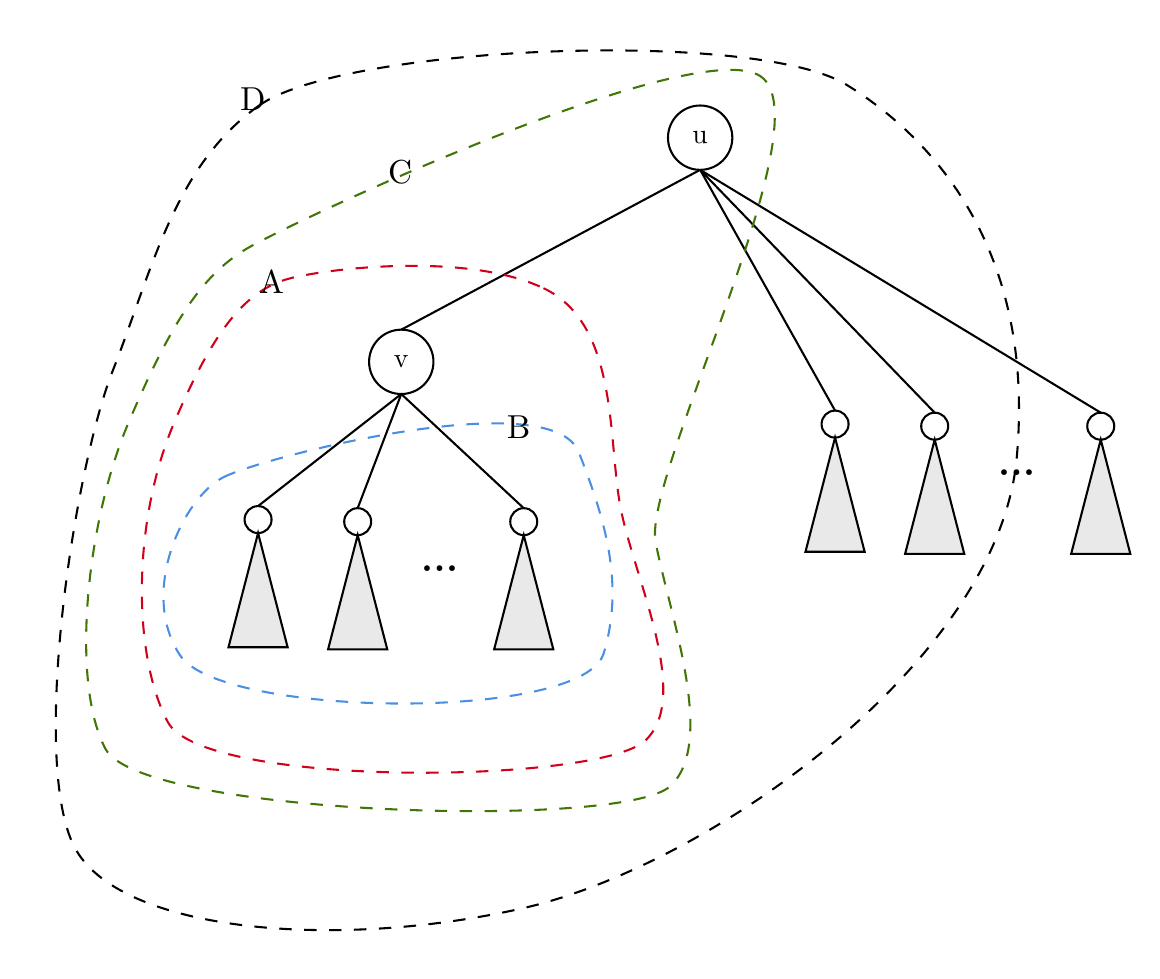
\begin{tikzpicture}[x=0.75pt,y=0.75pt,yscale=-1,xscale=1]
        %uncomment if require: \path (0,459); %set diagram left start at 0, and has height of 459

        %Shape: Circle [id:dp7711684678996311]
        \draw  [fill={rgb, 255:red, 255; green, 255; blue, 255 }  ,fill opacity=1 ] (302,48.5) .. controls (302,39.94) and (308.94,33) .. (317.5,33) .. controls (326.06,33) and (333,39.94) .. (333,48.5) .. controls (333,57.06) and (326.06,64) .. (317.5,64) .. controls (308.94,64) and (302,57.06) .. (302,48.5) -- cycle ;
        %Shape: Circle [id:dp8540052293183187]
        \draw  [fill={rgb, 255:red, 255; green, 255; blue, 255 }  ,fill opacity=1 ] (158,156.5) .. controls (158,147.94) and (164.94,141) .. (173.5,141) .. controls (182.06,141) and (189,147.94) .. (189,156.5) .. controls (189,165.06) and (182.06,172) .. (173.5,172) .. controls (164.94,172) and (158,165.06) .. (158,156.5) -- cycle ;
        %Shape: Circle [id:dp6767312206403671]
        \draw   (98,232.5) .. controls (98,228.91) and (100.91,226) .. (104.5,226) .. controls (108.09,226) and (111,228.91) .. (111,232.5) .. controls (111,236.09) and (108.09,239) .. (104.5,239) .. controls (100.91,239) and (98,236.09) .. (98,232.5) -- cycle ;
        %Shape: Triangle [id:dp6284155562718452]
        \draw  [fill={rgb, 255:red, 233; green, 233; blue, 233 }  ,fill opacity=1 ] (104.5,239) -- (118.75,294) -- (90.25,294) -- cycle ;
        %Shape: Circle [id:dp024913106678187136]
        \draw   (146,233.5) .. controls (146,229.91) and (148.91,227) .. (152.5,227) .. controls (156.09,227) and (159,229.91) .. (159,233.5) .. controls (159,237.09) and (156.09,240) .. (152.5,240) .. controls (148.91,240) and (146,237.09) .. (146,233.5) -- cycle ;
        %Shape: Triangle [id:dp11973699329342047]
        \draw  [fill={rgb, 255:red, 233; green, 233; blue, 233 }  ,fill opacity=1 ] (152.5,240) -- (166.75,295) -- (138.25,295) -- cycle ;
        %Shape: Circle [id:dp5828391286835717]
        \draw   (226,233.5) .. controls (226,229.91) and (228.91,227) .. (232.5,227) .. controls (236.09,227) and (239,229.91) .. (239,233.5) .. controls (239,237.09) and (236.09,240) .. (232.5,240) .. controls (228.91,240) and (226,237.09) .. (226,233.5) -- cycle ;
        %Shape: Triangle [id:dp2511681856589991]
        \draw  [fill={rgb, 255:red, 233; green, 233; blue, 233 }  ,fill opacity=1 ] (232.5,240) -- (246.75,295) -- (218.25,295) -- cycle ;
        %Shape: Circle [id:dp5623627355443772]
        \draw   (376,186.5) .. controls (376,182.91) and (378.91,180) .. (382.5,180) .. controls (386.09,180) and (389,182.91) .. (389,186.5) .. controls (389,190.09) and (386.09,193) .. (382.5,193) .. controls (378.91,193) and (376,190.09) .. (376,186.5) -- cycle ;
        %Shape: Triangle [id:dp39244508786141674]
        \draw  [fill={rgb, 255:red, 233; green, 233; blue, 233 }  ,fill opacity=1 ] (382.5,193) -- (396.75,248) -- (368.25,248) -- cycle ;
        %Shape: Circle [id:dp8178713595847904]
        \draw   (424,187.5) .. controls (424,183.91) and (426.91,181) .. (430.5,181) .. controls (434.09,181) and (437,183.91) .. (437,187.5) .. controls (437,191.09) and (434.09,194) .. (430.5,194) .. controls (426.91,194) and (424,191.09) .. (424,187.5) -- cycle ;
        %Shape: Triangle [id:dp3542102499533475]
        \draw  [fill={rgb, 255:red, 233; green, 233; blue, 233 }  ,fill opacity=1 ] (430.5,194) -- (444.75,249) -- (416.25,249) -- cycle ;
        %Shape: Circle [id:dp4483381477394748]
        \draw   (504,187.5) .. controls (504,183.91) and (506.91,181) .. (510.5,181) .. controls (514.09,181) and (517,183.91) .. (517,187.5) .. controls (517,191.09) and (514.09,194) .. (510.5,194) .. controls (506.91,194) and (504,191.09) .. (504,187.5) -- cycle ;
        %Shape: Triangle [id:dp4240387998981314]
        \draw  [fill={rgb, 255:red, 233; green, 233; blue, 233 }  ,fill opacity=1 ] (510.5,194) -- (524.75,249) -- (496.25,249) -- cycle ;
        %Straight Lines [id:da29060880873239037]
        \draw    (317.5,64) -- (173.5,141) ;


        %Straight Lines [id:da681996043601955]
        \draw    (317.5,64) -- (382.5,180) ;


        %Straight Lines [id:da7335165640252448]
        \draw    (317.5,64) -- (430.5,181) ;


        %Straight Lines [id:da39989551498039266]
        \draw    (317.5,64) -- (510.5,181) ;


        %Straight Lines [id:da27519719998677683]
        \draw    (104.5,226) -- (173.5,172) ;


        %Straight Lines [id:da1425001048459873]
        \draw    (152.5,227) -- (173.5,172) ;


        %Straight Lines [id:da8004516890426716]
        \draw    (232.5,227) -- (173.5,172) ;


        %Shape: Polygon Curved [id:ds10919181429761804]
        \draw  [color={rgb, 255:red, 208; green, 2; blue, 27 }  ,draw opacity=1 ][dash pattern={on 4.5pt off 4.5pt}] (242,121) .. controls (278,138) and (273,193) .. (279,226) .. controls (285,259) and (314,318) .. (291,339) .. controls (268,360) and (78,362) .. (61,330) .. controls (44,298) and (43.75,233.63) .. (64,186) .. controls (84.25,138.38) and (100,121) .. (121,116) .. controls (142,111) and (206,104) .. (242,121) -- cycle ;
        %Shape: Polygon Curved [id:ds3630985664957256]
        \draw  [color={rgb, 255:red, 74; green, 144; blue, 226 }  ,draw opacity=1 ][dash pattern={on 4.5pt off 4.5pt}] (88,212) .. controls (108,202) and (246,167) .. (259,200) .. controls (272,233) and (281,264) .. (271,297) .. controls (261,330) and (87,328) .. (67,298) .. controls (47,268) and (68,222) .. (88,212) -- cycle ;
        %Shape: Polygon Curved [id:ds6625985709394309]
        \draw  [color={rgb, 255:red, 65; green, 117; blue, 5 }  ,draw opacity=1 ][dash pattern={on 4.5pt off 4.5pt}] (345,18) .. controls (381,35) and (290,210) .. (296,243) .. controls (302,276) and (326,340) .. (303,361) .. controls (280,382) and (48,375) .. (31,343) .. controls (14,311) and (21.75,233.63) .. (42,186) .. controls (62.25,138.38) and (77,115) .. (99,102) .. controls (121,89) and (309,1) .. (345,18) -- cycle ;
        %Shape: Polygon Curved [id:ds5228551783856155]
        \draw  [color={rgb, 255:red, 0; green, 0; blue, 0 }  ,draw opacity=1 ][dash pattern={on 4.5pt off 4.5pt}] (105,33) .. controls (146,4) and (344,-4) .. (388,23) .. controls (432,50) and (479,105) .. (470,203) .. controls (461,301) and (321,400) .. (231,420) .. controls (141,440) and (40,431) .. (17,392) .. controls (-6,353) and (15.5,209) .. (34.5,160.75) .. controls (53.5,112.5) and (64,62) .. (105,33) -- cycle ;

        % Text Node
        \draw (317.5,48.5) node  [align=left] {u};
        % Text Node
        \draw (173.5,156.5) node  [align=left] {v};
        % Text Node
        \draw (192,256) node  [align=left] {\textbf{{\Large ...}}};
        % Text Node
        \draw (470,210) node  [align=left] {\textbf{{\Large ...}}};
        % Text Node
        \draw (111,118) node [scale=1.2] [align=left] {A};
        % Text Node
        \draw (230,188) node [scale=1.2] [align=left] {B};
        % Text Node
        \draw (173,65) node [scale=1.2] [align=left] {C};
        % Text Node
        \draw (102,30) node [scale=1.2] [align=left] {D};


    \end{tikzpicture}

    \caption{Different cut types for the decompose algorithm}\label{fig:decompose}
\end{figure}